%%%%%%%%%%%%%%%%%%%%%%%%%%%%%%%%%%%%%%%%%
% Short Sectioned Assignment LaTeX Template Version 1.0 (5/5/12)
% This template has been downloaded from: http://www.LaTeXTemplates.com
% Original author:  Frits Wenneker (http://www.howtotex.com)
% License: CC BY-NC-SA 3.0 (http://creativecommons.org/licenses/by-nc-sa/3.0/)
%%%%%%%%%%%%%%%%%%%%%%%%%%%%%%%%%%%%%%%%%

%----------------------------------------------------------------------------------------
%	PACKAGES AND OTHER DOCUMENT CONFIGURATIONS
%----------------------------------------------------------------------------------------

\documentclass[paper=a4, fontsize=10pt]{article} % A4 paper and 11pt font size


\usepackage[vmargin=2.5cm,hmargin=3cm]{geometry}
% ---- Entrada y salida de texto -----

\usepackage[T1]{fontenc} % Use 8-bit encoding that has 256 glyphs
\usepackage[utf8]{inputenc}
\usepackage{helvet}
\renewcommand{\familydefault}{\sfdefault}
%\usepackage{fourier} % Use the Adobe Utopia font for the document - comment this line to return to the LaTeX default

% ---- Idioma --------

\usepackage[spanish, es-tabla]{babel} % Selecciona el español para palabras introducidas automáticamente, p.ej. "septiembre" en la fecha y especifica que se use la palabra Tabla en vez de Cuadro

% ---- Otros paquetes ----
\usepackage[hidelinks]{hyperref} % Estilo para los enlaces
\hypersetup{
  colorlinks   = true, %Colours links instead of ugly boxes
  urlcolor     = blue, %Colour for external hyperlinks
  linkcolor    = black, %Colour of internal links
  citecolor   = blue %Colour of citations
}
\usepackage{url} % ,href} %para incluir URLs e hipervínculos dentro del texto (aunque hay que instalar href)
\usepackage{amsmath,amsfonts,amsthm} % Math packages
%\usepackage{graphics,graphicx, floatrow} %para incluir imágenes y notas en las imágenes
\usepackage{graphics,graphicx, float} %para incluir imágenes y colocarlas

%Para incluir codigo
\usepackage{minted}

% Para hacer tablas comlejas
%\usepackage{multirow}
%\usepackage{threeparttable}

%\usepackage{sectsty} % Allows customizing section commands
%\allsectionsfont{\centering \normalfont\scshape} % Make all sections centered, the default font and small caps

\usepackage{fancyhdr} % Custom headers and footers
\pagestyle{fancyplain} % Makes all pages in the document conform to the custom headers and footers
\fancyhead{} % No page header - if you want one, create it in the same way as the footers below
\fancyfoot[L]{} % Empty left footer
\fancyfoot[C]{} % Empty center footer
\fancyfoot[R]{\thepage} % Page numbering for right footer
\renewcommand{\headrulewidth}{0pt} % Remove header underlines
\renewcommand{\footrulewidth}{0pt} % Remove footer underlines
\setlength{\headheight}{13.6pt} % Customize the height of the header

\numberwithin{equation}{section} % Number equations within sections (i.e. 1.1, 1.2, 2.1, 2.2 instead of 1, 2, 3, 4)
\numberwithin{figure}{section} % Number figures within sections (i.e. 1.1, 1.2, 2.1, 2.2 instead of 1, 2, 3, 4)
\numberwithin{table}{section} % Number tables within sections (i.e. 1.1, 1.2, 2.1, 2.2 instead of 1, 2, 3, 4)

\setlength\parindent{0pt} % Removes all indentation from paragraphs - comment this line for an assignment with lots of text

\newcommand{\horrule}[1]{\rule{\linewidth}{#1}} % Create horizontal rule command with 1 argument of height


%----------------------------------------------------------------------------------------
%	TÍTULO Y DATOS DEL ALUMNO
%----------------------------------------------------------------------------------------

\title{	
\normalfont \normalsize 
\textsc{\textbf{Ingeniería de Servidores (2016-2017)} \\ Grado en Ingeniería Informática \\ Universidad de Granada} \\ [25pt] % Your university, school and/or department name(s)
\horrule{0.5pt} \\[0.4cm] % Thin top horizontal rule
\huge Memoria \\ % The assignment title
\horrule{2pt} \\[0.5cm] % Thick bottom horizontal rule
}

\author{Elena María Gómez Ríos y Jose Luis Martínez Ortiz} % Nombre y apellidos

\date{\normalsize\today} % Incluye la fecha actual

%----------------------------------------------------------------------------------------
% DOCUMENTO
%----------------------------------------------------------------------------------------

\begin{document}

\maketitle % Muestra el Título

\newpage %inserta un salto de página

\tableofcontents % para generar el índice de contenidos

\listoffigures

\listoftables

\newpage

%\textbf{NOTA: en caso de problema al compilar, compruebe que tiene el paquete: texlive-babel-spanish.noarch }  \\
 
\newpage

%----------------------------------------------------------------------------------------
%	Resumen introductorio
%----------------------------------------------------------------------------------------

\section{Resumen}


%----------------------------------------------------------------------------------------
%	Introducción
%----------------------------------------------------------------------------------------

\section{Introducción}


%----------------------------------------------------------------------------------------
%	Systemd
%----------------------------------------------------------------------------------------

\section{Systemd}


%----------------------------------------------------------------------------------------
%	Conclusiones
%----------------------------------------------------------------------------------------

\section{Conclusiones}

\begin{figure}[H] %con el [H] le obligamos a situar aquí la figura
\centering
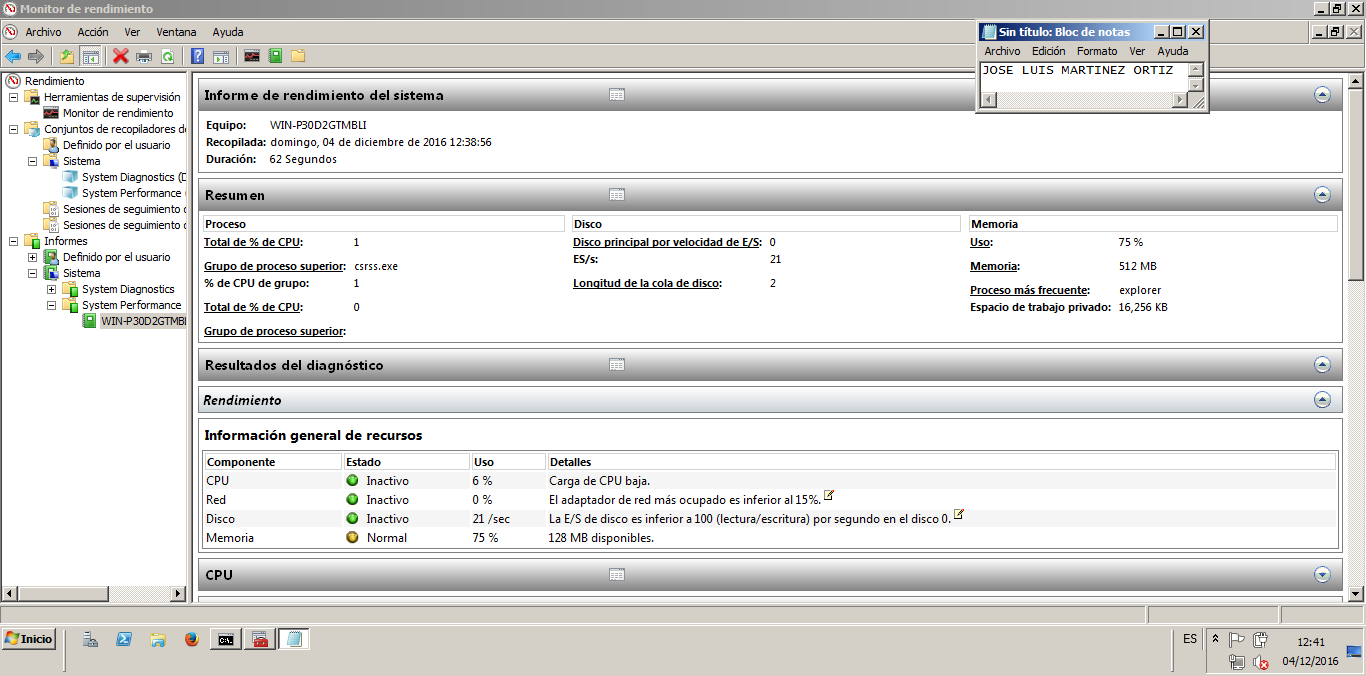
\includegraphics[scale=0.4]{./imagenes/P3_4_1.png} 
\caption{Informe del monitor de rendimiento - resumen} \label{fig:P3_4_1}
\end{figure}


%----------------------------------------------------------------------------------------
%	Tareas extra
%----------------------------------------------------------------------------------------
\section{Tareas extra.}


\subsection{Instalación y utilización de lm-sensors}
Para probar el software que se indica en el guión de prácticas \textit{lm-sensor} consulto 
la wiki de Arch \cite{lmSensor}, ya que la web indicada en el guión no esta operativa.
Lo realizo sobre mi propio equipo ya que en las máquinas virtuales no cuentan con los sensores de
las BIOS.
Como se puede ver en la imagen \ref{fig:P3_E2_1} ya tengo instalado el software. Ahora paso a 
configurar a que sensores de mi equipo le doy acceso para monitorizar (figura \ref{fig:P3_E2_2}).
Una vez configurado los permisos ya podemos ver la información mediante el comando \textit{sensors},
tal como se ve en la figura \ref{fig:P3_E2_3}.\\

Podemos ver como la temperatura de los ``cores'' esta en valores normales, además nos indica que por
encima de 81º es una temperatura alta y por encima de los 105º ya es critica. También nos informa de la
velocidad del ventilador del equipo, en nuestro caso esta funcionando a 27000 rpm (revoluciones por minuto)




%------------------------------------------------

\bibliography{citas} %archivo citas.bib que contiene las entradas 
\bibliographystyle{plain} % hay varias formas de citar

\end{document}



